\documentclass[conference,a4]{IEEEtran}
\IEEEoverridecommandlockouts
% The preceding line is only needed to identify funding in the first footnote. If that is unneeded, please comment it out.
\usepackage{cite}
\usepackage{amsmath,amssymb,amsfonts}
\usepackage{algorithmic}
\usepackage{graphicx}
\usepackage{textcomp}
\usepackage{xcolor}
\def\BibTeX{{\rm B\kern-.05em{\sc i\kern-.025em b}\kern-.08em
    T\kern-.1667em\lower.7ex\hbox{E}\kern-.125emX}}
\usepackage{flushend}

\usepackage{luatextra}
\usepackage{currvita}
%
\usepackage{makeidx}  % allows for indexgeneration
\usepackage{url}
\usepackage{doi}
%\usepackage[biblabel]{cite}
%\usepackage{amsmath,amssymb,amsfonts}
%\usepackage{algorithmic}
%\usepackage{graphicx}
%\usepackage[pdftex]{graphicx}
%\usepackage[dvips]{graphicx}
\usepackage{alltt}
%\usepackage{textcomp}
\usepackage{enumitem}
\usepackage{minted}
%\usepackage{indentfirst}

%
% Used for displaying a sample figure. If possible, figure files should
% be included in EPS format.
%
% If you use the hyperref package, please uncomment the following line
% to display URLs in blue roman font according to Springer's eBook style:
% \renewcommand\UrlFont{\color{blue}\rmfamily}


\usepackage{hyperref}
\hypersetup{
    % bookmarks=true,         % show bookmarks bar?
    unicode=true,          % non-Latin characters in Acrobat’s bookmarks
    pdftoolbar=true,        % show Acrobat’s toolbar?
    pdfmenubar=true,        % show Acrobat’s menu?
    pdffitwindow=false,     % window fit to page when opened
    pdfstartview={FitH},    % fits the width of the page to the window
    %pdftitle={},    % title
    %pdfauthor={Author},     % author
    %pdfsubject={Subject},   % subject of the document
    %pdfcreator={Creator},   % creator of the document
    %pdfproducer={Producer}, % producer of the document
    %pdfkeywords={keyword1, key2, key3}, % list of keywords
    %pdfnewwindow=true,      % links in new PDF window
    colorlinks=true,       % false: boxed links; true: colored links
    linkcolor=black,          % color of internal links (change box color with linkbordercolor)
    citecolor=black,        % color of links to bibliography
    filecolor=black,      % color of file links
    urlcolor=black,           % color of external links
    final=true
  }

\setmainfont{Times New Roman}
\renewcommand{\doitext}{DOI:}
\begin{document}

% \title{Recommender system for high school entrants having social network accounts}

\title{Recommender systems for carer guidance}

\author{%
\IEEEauthorblockN{Trần Đức Thế${}^{1}$, Viktoria Kopylova${}^1$, Evgeny Cherkashin${}^{1,2,3}$, Nikita Lukyanov${}^1$}
\IEEEauthorblockA{${}^1$~\textit{Institute for Informational Technologies and Data Analysis},\\
\textit{National Research Irkutsk State Technical University,} Irkutsk, Russia}
\IEEEauthorblockA{${}^2$~\textit{Laboratory of Complex Informational Systems},\\\textit{Matrosov Institute for System Dynamics and Control Theory, Siberian Branch of Russian Academy of Sciences,}
Irkutsk, Russia}
\IEEEauthorblockA{${}^3$~\textit{Chair for Informational Technologies},\\\textit{Institute for Mathematics and Information Technologies, Irkutsk State University, Irkutsk, Russia}\\ \emph{eugeneai@icc.ru}}
}

\newcommand{\irnitu}{INRTU}
\newcommand{\inrtu}{INRTU}

\maketitle
% \onecolumn
\begin{abstract}
  The research of the paper is devoted to present of an R\&D of two recommender systems in carer guidance for Việt Nam middle school students and one for testing a paper \cite{tomsk} technique for data obtained in National research Irkutsk state technical university (\irnitu).  The first system is built on the base of John Holland's six personality types theory and collecting university students' opinions on their study conditions, and the second one relates data from a social network and faculty enrollment documents.  Both systems describe new user (an entrant or a pupil) properties by distances to student groups and then presents top-$N$ universities/departments as a recommendation.  Techniques of overcoming ``cold start'' problem and other ones in this domain are considered.

  % This paper deals with mostly with the stage of information acquisition, correlation patterns construction and taxonomy construction for entrants and high school subjects.
\end{abstract}

\begin{IEEEkeywords}
recommender system, cold start, carer guidance, user group description, machine learning
\end{IEEEkeywords}

\section{Introduction}

In the countries with predominantly young population, such as Việt Nam, the demand of young specialists is high.  While still a high school student, one have to make a decision about a career. Career choice depends on many factors such as personal interests, academic ability and employment opportunities available after the graduation.  Therefore, choosing the right carer is not an easy task.  In fact, quite often graduates remain unemployed for a long time or do not work in their specialties mastered in an educational institution.  This leads to inefficient use of state funds, their irrational distribution.  That's why the choice of an university after receiving a certificate of maturity is very important.  Choosing a suitable university results in an increase students' study productively, as they work and practice with enthusiasm.  Supporting the decision activities will give a better chance of achieving students' goals in the future.

In Tables 1 and 2, we present the result of interest assessment to career guidance and relevance of improving of the guidance system.  Tables show that there is a real problem of carer guidance and middle school students are very interested in improving the corresponding activities.
\begin{table}[thb]
  \caption{Interest assessment to the career guidance in Việt Nam, Hà Tĩnh city}
  \label{tab:interest}
  \centering
  \begin{tabular}{|l|c|c|}
    \hline
    \textbf{Interest level} & \textbf{Count of votes} & \textbf{Ratio, \%} \\
    \hline
    Very interested & 218 & 51.9 \\
    \hline
    Relatively interested & 155 & 36.9 \\
    \hline
    Less interested & 36 & 8.6 \\
    \hline
    No interest & 11 & 2.6 \\
    \textbf{Total} & \textbf{420} & \textbf{100} \\
    \hline
  \end{tabular}
\end{table}

\begin{table}[bht]
  \caption{Questionary results of middle school students on need for improvement of the career guidance system}
  \label{tab:interest}
  \centering
  \begin{tabular}{|l|c|c|}
    \hline
    \textbf{Answer option} & \textbf{Quantity} & \textbf{Ratio, \%} \\
    \hline
    very necessary & 272 & 64.8 \\
    \hline
    necessary & 145 & 34.5 \\
    \hline
    no necessity & 3 & 0.7 \\
    \hline
    \textbf{Total} & \textbf{420} & \textbf{100} \\
    \hline
  \end{tabular}
\end{table}

At present, with the development of the Internet, the search for information about universities is sufficiently efficient. However, having a huge amount of information, selecting substantive information is a difficult task.  Recommender systems (RS) have emerged as a decision support tool, providing users with the most useful and personalized variants for goods and services.  The functioning of RS is based on filtering information with respect to a set of known properties of objects and users.  For example, RSs are used to assess the users' preferences for goods and services (songs, films, video clips, books, articles, \emph{etc}.), which have been not previously given ratings by the user trying to make a choice.

RSs are also quite successfully used in many business spheres, such as entertainment: offering songs to listeners (\emph{e.g.}, the LastFM system -- www.last.fm), offering films (the Netflix system -- www.netflix.com), recommended videos (the YouTube system -- www.youtube.com); in education and training (learning resources, books, articles, site addresses), in intelligent systems of teacher assistants (predicting students' learning capabilities).  RSs are the field of active IT research since 2007.  Our literature and technologies review is in~\cite{review}.

Teaching experience of the first author of this paper in secondary school shows the relevance of the problem of choice of a profession.  This research, being the results of a master thesis, is dedicated to the development of an RS that allows students (applicants) to receive recommendations when taking career decisions.  The aim of the research is development of RSs for supporting students in their carer decision making and for universities management staff to analyze actual demand and elaborate the best sets of courses.

The resulting RS prototypes have various options for producing recommendations. The first one is realized on the base of John Holland theory~\cite{holland}, according to which most people have one of six personality types.  After determining the type, a set of corresponding universities are produced.  The second one is an aggregation of questioning data about concrete universities obtained from students already being taught there.  The third option is acquisition of user profile and subscription data from a social network and enrollment documents of a university.  The obtained data is processed to construct taxonomies and class recognition procedures.  The recommendations, then, are generated by means of collaborative filtration (CF) based on users' RS profile comparison.

\section{Technique of data collection}
\label{sec:base}

\emph{Recommender systems}~\cite{rs_basics} are decision support information systems designed to assess the user's level of interest in a particular product or service (object) based on available information about user and object.  The RS development industry began to actively develop with the emergence of online sales services, and now it is one of the active areas of development of decision support systems, a direction of artificial intelligence, focused primarily on commercial use, as well as on solving problems of increasing the productivity of searching for relevant information.  A profession is the object of RS recommendation production.  Let us consider the development technique for RS construction from the point of view of solving the standard set problems and challenges.


Development of the RSs is aimed at solving the following set of problems \cite{ricci}:
\begin{enumerate}
\item Increasing the sales of a product
  \begin{itemize}
  \item a number of commodities sold,
  \item organizing wider range product sales;
  \end{itemize}
\item Increasing user satisfaction and/or loyalty;
\item Better understanding user needs;
\item Better products offers with respect to the user needs;
\item Selection of sets of products for users with a common properties
  \begin{itemize}
  \item ``good'' ones, and
  \item product groups, having a common usability properties;
  \end{itemize}
\item Mining the classes of products, structuring the RS product domain, and
\item Generate a continuity of recommendations using the classification;
\item Rectifying user profile, \emph{e.g.} with targeted questioning;
\item For the users having no goal to make choice, but searching for an expert opinions,
  \begin{itemize}
  \item Analysis of other users impact on a choice,
  \item Formalizing opinions,
  \item Recommending opinions.
  \end{itemize}
\end{enumerate}
In this context, the first RS (for Viet Nam students) is aimed at solving 4--7-th problems.  This set defines the methods of RS proposal generation and algorithms, which have to be implemented.  As we can see, the universities and their departments can be distributed on various carer directions by two ways: with the use of expert knowledge, when experts analyze a departments' properties and relate them to a direction, and with use of opinions of the students (users who already ``consume'' a product).  A good opinion of a user on a department (product) creates or solidifies a corresponding relation.  In the same time, a group of students positively characterized a department form a group of ``similar'' users.  % A new user, \emph{i.e.}, an enrollee of a middle school student, is to be tested with John Holland's theory to gain initial profile data.
The second RS aimed at solving problems~1, 6, 7, 9 as almost all algorithms are developed for acquire and structure information for further decision production in a general form.

The main problem solved during the R\&D is ``\emph{cold-start}'' \emph{problem}.  For RS based on CF, the similarity of user profiles in terms of sets of specified characteristics are performed. Content filtering RS compare products. In both cases, RS cannot generate recommendations if it does not have enough information about users or products.  The cold-start problem arises at the first stages of RS functioning and when a new user's behavior had not been observed sufficient time, \emph{i.e.}, the RS have no data about his preferences, or user's profile contains no useful information for a comparison.  The same situations arises for a new product, \emph{e.g.} there is no user bought the product, and no responses were given.  In the first system explicit information collection has been realized for solving cold-start problem in CF, and John Holland's theory was used as initial profile data filling in, including the input data for the Holland's questionary.

The simplest technique for user profile data collection and usage is so called \emph{impersonalized acquisition}.  Recommendations are generated for an ``average'' user related to a nearest group od users.  An RS gives top-$N$ products for the group, efficiently ignoring personal preferences.  The approach can be developed to support personal data with construction of subgroups of the groups relating them to a set of personal characteristics.  This may lead to unwillingness giving personal data of users and impossibility to generate proposals when a user cardinally changes his/her preferences.  In this system, as our intention is a detection of a direction of a carer, impersonalized approach seems to give sufficient quality result.

\subsection{Holland's six types TODO}

Realistic, Investigative, Artistic, Social, Enterprising, Conventional. % Pages 27 of thesis

In order to determine the type one must answer 54 questions, the questions are evenly distributed on this six types.  For each question, a 0-4 scores are to be set depending on the degree of manifestation. The store 0 corresponds to ``no manifestation'' was mentioned of a kind, and score 4 denotes ``always manifestative''.  For each type the scores of the corresponding nine questions are collected, and the type is figured out as a type with the maximum score sum.  Student profiles store all answers and estimates, just for a further system development.

\subsection{Collecting data from social network and enrollment documents}
\label{sec:collect-2}

Social networks allow one to track the self-expression, interests and attitude to the world of each person by analyzing subscription groups, posts and reposts, statuses, \emph{etc} \cite{kb7}.  This tendency is especially exposed by schoolchildren and students, who, according to the research of Tomsk State University (TSU) \cite{kb20}, update subscriptions every six months or a year as irrelevant content in the feed annoys them. Therefore, it can be assumed that user subscriptions to certain topics really reflect his interests and can serve as a starting point for a deeper analysis.  The personal social page in a network, entrants inform university staff on a request.

In 2016, TSU showed that the social network ``In~Contact'' (in~Russian -- ``В~Контакте'') profile reflects the cognitive personality traits, \emph{i.e.}, the educational interests of schoolchildren are closely related to their behavior in the social network \cite{kb9}.  Applying this technique for \irnitu{} data, the similar results should to be obtained.  Object data for the RS were obtained by parsing enrollment documents for each department of \irnitu.  The documents contain lists of students, and these list were used to search their social network accounts for further analysis.

\vspace{0.7em}
% \begin{center}
%   \hbox{*~*~*}
% \end{center}
% \vspace{1em}

The \emph{scalability problem}. Scalability is a property of software systems to be able to cope with the load prescribed by design, as well as with increased load if additional information--communication and computing resources are available.  For a simple RS with several users and products, there is no need to maintain scalability, and algorithms such as ``nearest-neighbor'' are widely used for assessing interests as the combinatorial space is not large. % TODO: SAY what algos used...

Thus, to construct carer choice RS prototype, different ways to collect data in the RSs were chosen: the first one collected impersonalized data, in the same time, the second RS collects highly personalized data.  The collected impersonalized user data were structured with respect to university/department preference and user profiles by means of collaborative filtering, use questionary and expert approach for initial user profile filling in.

\section{Database structure}

\begin{figure}\centering

  \includegraphics[width=\linewidth]{pics/2-obj-stru.png}

  \caption{The structure of the second RS}
  \label{fig:2-struct}
\end{figure}
\section{Implementation}

Both RS are MVC\footnote{Abbreviation of Model-View-Controller programming pattern} web-applications, the first one is realized with Django and the second one with ASP.NET.

The Django RS uses MySQL for data storage.  Python programming language is the main glue subsystem, gathering web-application and recommender unit in one system.  For carrying out experiments with data, a Jupiter subsystem was included in the system as well.

User roles are administrators, anonymous and regular user.  Administrator can manipulate user accounts and any raw data.  Anonymous users can register, view information on universities, taught courses and professions.  Regular registered user can obtain recommendations, rate universities, add an university to his/her preference list.  The use-case diagram is shown in Figure~\ref{fig:use-case}.
\begin{figure}[tb]
  \centering
  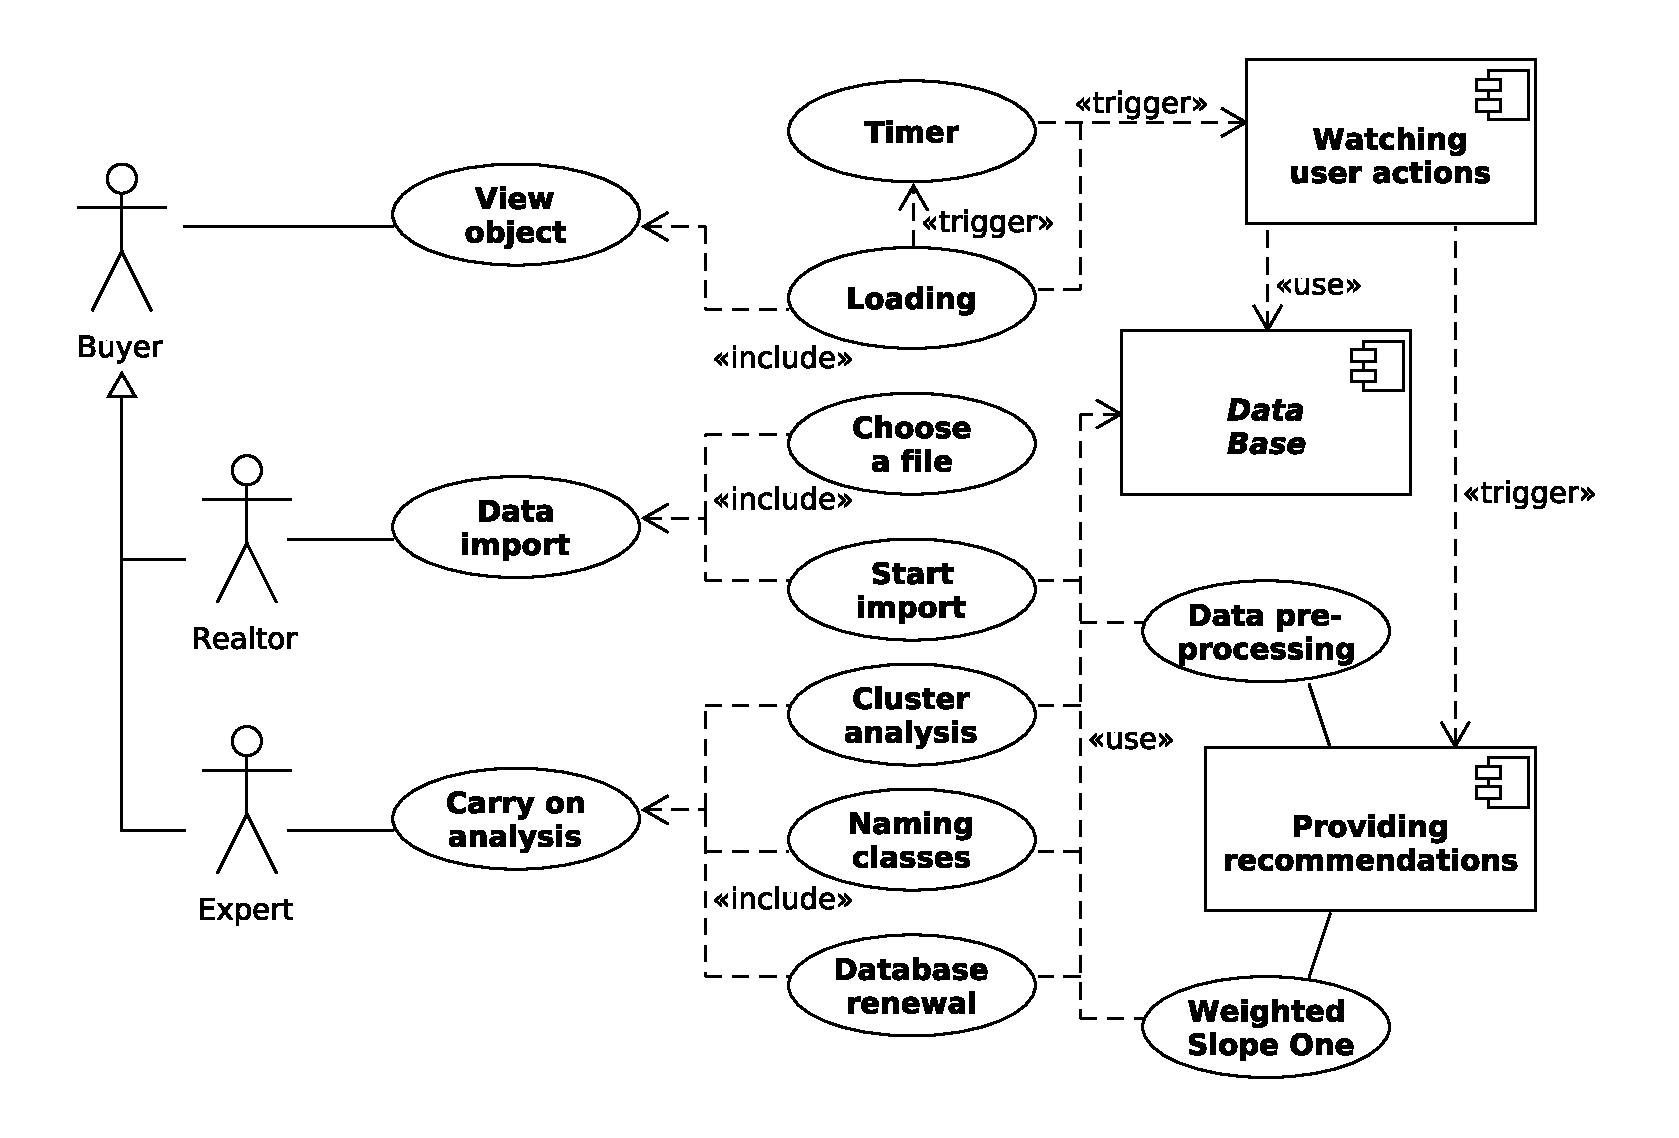
\includegraphics[width=\linewidth]{use_case.eps}
  \caption{Use case diagram for real estate RS [TODO: UPDATE to CDT's thesis]}  % Page 57
  \label{fig:use-case}
\end{figure}

\begin{minted}[fontsize=\footnotesize]{python}
from django.db import models
from django.contrib.auth.models import AbstractUser

# User
class NGUOIDUNG(models.Model):
IdUser = models.AutoField(primary_key=True)
TenNguoiDung = models.CharField(max_length=20, null=False)
HoTen = models.CharField(max_length=200, null=False)
MatKhau = models.CharField(max_length=200, null=False)
Email = models.CharField(max_length=200, null=False)
Quyen = models.IntegerField(null=False)
GioiTinh = models.BooleanField(default=False)
SDT = models.CharField(max_length=15, null=True)
NgaySinh = models.DateTimeField(null=False,
  default="1999-01-01")

# Interests
class TINHCACH(models.Model):
IdTinhCach = models.AutoField(primary_key=True)
Loai = models.IntegerField(null = False)
ChiTiet = models.CharField(max_length=1000, null=False)
# List university

class TRUONG(models.Model):
IdTruong = models.AutoField(primary_key=True)
TenTruong = models.CharField(max_length=1000, null=False,default="")
ChiTiet = models.CharField(max_length=1000, null=True)
ChiTietFull = models.CharField(max_length=1000, null=True)

# Vote for an university
class VOTE(models.Model):
IdVote = models.AutoField(primary_key=True)
IdTruong = models.IntegerField(null=False)
IdUser = models.IntegerField(null=False)
Point = models.IntegerField(default=0)

# List of favorite universities
class FAVORITE(models.Model):
IdFavo = models.AutoField(primary_key=True)
IdTruong = models.IntegerField(null=False)
IdUser = models.IntegerField(null=False)
\end{minted}

For representing answers on Holland's questionary and intermediate data two tables added.

\begin{minted}[fontsize=\footnotesize]{python}
from django.db import models
# Create your models here.
class ListUni(models.Model):
name = models.CharField(max_length=100)
description = models.TextField()
excerpt = models.TextField(max_length=300)
pictrure = models.ImageField(upload_to='Uni_picture')
group = models.IntegerField(default=0)
def __str__(self):
return self.name
class list1(models.Model):
name = models.CharField(max_length=100)
anddress = models.CharField(max_length=200)
description = models.TextField()
excerpt = models.TextField(max_length=300)
pictrure = models.ImageField(upload_to='Uni_picture')
group = models.IntegerField(default=0)
def __str__(self):
return self.name
\end{minted}


TODO Activity diagram % Page 58, 59 - 61

The second ASP.NET RS uses Microsoft SQL Server as database server and Entity Framework for the database structure representation.

\section{Preliminary Data Processing}
\label{sec:relim-proc}

\subsection{Analysis of social network data}
\label{sec:socnetan}

For bachelors and specialists entrants, the last three year data from ``In~Contect'' were loaded.  For 6270 enrolled students, the data were found for 4325 (68.98\%) ones of them.  The input was represented as \texttt{.CSV}-file with 4325 rows and 480 columns.  After that a part of profiles were filtered outs due to user mark ``private'', and the same has been done for columns for topics, blocked by Russian government (extremism and similar ones).  After this cleansing, the table comprised only 686 rows and 389 columns, including \texttt{CategoryID}, the identifier of a category (institute of \irnitu), \texttt{StudentID}, \texttt{CountFriends}, \texttt{CountFollowers}, \texttt{CountNotes}, the number of the messages the user wrote, \texttt{CountPhotos}.  The distribution of the students, whose accounts contain sensible data, between institutes of \irnitu{} is shown in Table~\ref{tab:numstudbycat}.

\begin{table}
  \caption{Number of students by categories}
  \label{tab:numstudbycat}
  \centering
  \begin{tabular}{|l|c|}
    \hline
    \textbf{Institute} & \textbf{Number of students} \\
    \hline
   ИАМиТ & 101\\
   ИАСиД & 137\\
   ИВТ & 81\\
   ИН & 167\\
   ИЭ  & 48\\
   ИЭУиП & 77\\
           ИИТиАД & 75\\
                    \hline
  \end{tabular}
\end{table}



\section{Recommendations Generation}
\label{sec:proc-recs}


% Page 50 of the thesis



% The Slope One algorithm can generate recommendations for an object (a class) if there is at least one positive evaluation of an object of the class.  At the cold start period if there were no such evaluations, RS shows random 20 objects of the same class of objects user is viewing.

\section{Web Applications}

\section{Discussion}
\label{sec:disc}

Comparing these two approaches to the RS R\&D ....

The first approach ... allowed collecting data in the runtime of the RS and also used J.~Holland's theory, which has been used for decades for carer guidance, ...

The second approach ... is more useful for solving problems~1, 6,7,9 of the list of Section~\ref{sec:base}.



\section{Conclusion}
\label{sec:conc}

% Page 68

In this brief narration of the results of two master theses, information recommender systems (RS) were developed to support the choice of a profession for students in Viet Nam and Irkutsk, Russia. The following tasks have been solved:

1. The subject area of ​​RS, assistance in choosing a profession (carer guidance), have been analyzed; typical problems were recognized and their solution method were proposed.

2. The theory of John Holland in carer guidance was applied for high school students in Ki Lam High School, Ha Tinh, Viet Nam.

3. High school students of last courses tested the universities rating setting playing role of university students.

4. A methodology for calculating recommendations for carer guidance, based on the method of collaborative filtering and expert evaluation, is proposed.  The technique has been implemented with Python modules.

5. Implemented an RS subsystems in the Python programming environment based on the proposed techniques and data structures; This Rs was tested by younger students of the Viet Nam school.

The resulting RS MVP\footnote{Abbreviation of Minimal Valuable Product}, extended with automatic university data crawling and more efficient algorithms, is to be deployed in the school.

The source code is located at Github.com URL:~\url{https://github.com/tranducthe/diplom_CollaborativeFiltering}.


\section*{Acknowledgements}
\label{sec:ack}

The results were obtained within the state assignment of the Ministry of Education and Science of Russia, the project ``Methods and technologies of a cloud-based service-oriented digital platform for collecting, storing and processing large volumes of multi-format interdisciplinary data and knowledge based on the use of artificial intelligence, a model-driven approach and machine learning'', No.~FWEW-2021-0005 (State registration No.~121030500071-2).


% \section*{References}

\begin{thebibliography}{99}

\bibitem{tomsk} Tomsk hypothesis.
\bibitem{review} AIIT'2020 Cherkashin, et al. Two recommender ....
\bibitem{ricci} Ricci.... types of RSs.
\bibitem{rs_basics} D. Jannach, M. Zanker, A. Felfernig, G. Friedrich. Recommender Systems: An Introduction. Cambridge University Press, 2010.
\bibitem{RSPO}E.~Charkashin, B.~Shevchenko. Source code of a prototype real estate market recommender system.  URL:\url{https://github.com/eugeneai/RSPO-CSharp}. (access date: 21-09-2020)
\bibitem{br13} J. Beel, B. Gripp, S. Langer, C. Breitinger. Research-paper recommender systems: a literature survey. International Journal on Digital Libraries (2016) 17: 305. \doi{10.1007/s00799-015-0156-0}
\bibitem{c2}S.P.~Balandina, M.V.~Bautin, A.V.~Maiyorov, E.R.~Smirnova. Social networks as means of education and educational participants interactions. Pedagogicheskie i informacionniye tehnologii v obraxovanii. No. 15 (2016). (in Russian) URL:\url{https://journals.susu.ru/pit-edu/issue/view/31}
\bibitem{c6}K.S.~Veber, A.A.~Pimenova. Comparative analysis of social networks. Vestnik Tambovskogo universiteta. Series: Natural and technical sciences. Vol. 19, No. 2, 2014. p. 636--643. (in Russian)
\bibitem{c7}A.V.~Rozhkova. Self-expression (self-presentation) in social Internet networks as a phenomenon of human cyber-socialization. Homo Cyberus. 2017. No. 2(3). (in Russian) URL:\url{http://journal.homocyberus.ru/Samovyrazhenie_v_socialnyh_internet-setjah_kak_fenomen_kibersocializacii}
\bibitem{c11} A.V. Fescshenko. Social networks in education: experience analysis and development perspectives. Gumanitarnaya informatika, Tomsk, Issue 6. 2012. p. 124--134. (in Russian)
\bibitem{c9}V.V.~Matsuta, P.B. Kiselyev, A.V. Fescshenko, V.L. Goyko. Investigation of social networks potential for revealing talented students. Psychologiya i psihotehnika. No. 4. 2017. p. 104--121. (in Russian)
%\bibitem{wikiRS}Recommender system -- Wikipedia. URL:~\url{https://en.wikipedia.org/wiki/Recommender_system} (access date: 13.09.2020)
\bibitem{wb41}Ch.C. Aggarwal Recommender Systems: The Textbook. Springer. 2016. ISBN 9783319296579.
\bibitem{wb42}P. Brusilovsky. The Adaptive Web. 2007. p. 325. ISBN 978-3-540-72078-2.
\bibitem{wb43}D.H. Wang, Y.C. Liang, D.Xu, X.Y. Feng, R.C. Guan. "A content-based recommender system for computer science publications", Knowledge-Based Systems. 2018. 157: 1-9
\bibitem{wb44}S. Blanda. Online Recommender Systems – How Does a Website Know What I Want?. American Mathematical Society. 2015.
%\bibitem{wb45}X.Y. Feng, H. Zhang, Y.J. Ren, P.H. Shang, Y. Zhu, Y.C. Liang, R.C. Guan, D. Xu, The Deep Learning–Based Recommender System “Pubmender” for Choosing a Biomedical Publication Venue: Development and Validation Study, Journal of Medical Internet Research, 2019. 21 (5): e12957
\bibitem{ben16} J.~Albahari, B.~Albahari. C\#~6.0 in a Nutshell: The Definitive Reference 6th Edition, 2015. 1138~p. ISBN-13: 978-1491927069
\bibitem{ef15}Entity Framework Tutorial. URL:\url{https://www.entityframeworktutorial.net/} (access date: 05.07.2020).
\bibitem{apivk}VKontakte API documentation. URL: \url{https://vk.com/dev/manuals} (access date: 05.07.2020).
\bibitem{br1} D. Lemire, A. Maclachlan. Slope One Predictors for Online Rating-Based Collaborative. URL:~\url{http://cogprints.org/4031/1/lemiremaclachlan_sdm05.pdf} (access date: 10.05.2018)
\bibitem{friman15}A.~Freeman. Pro ASP.NET MVC 5. 5th ed. Apress. 2013. 832 p. \doi{10.1007/978-1-4302-6530-6}
\bibitem{cchadvik20} J. Chadwick, T. Snyder, H. Panda. Programming ASP.NET MVC 4: Developing Real-World Web Applications with ASP.NET MVC.  O'Reilly Media; 1st Edition. 2012. 492 p.  ISBN-13:~978-1449320317
\bibitem{br22}E. M. Alrawhani, H. Basirona, Z. Sa’ayaa. Real estate recommender system using case-based reasoning approach. Journal of
Telecommunication, Electronic and Computer Engineering (JTEC).
Vol. 8 No. 2. p. 177-182.
\bibitem{br20} E.~V.~Britina. Segmenting recommender system with client--server connection based on programmable configured networks and usage protocol with fast-jumping IP-address.  // Sovremennye problemy nauki i obrazovaniya. No 6. 2015.
URL:\url{https://www.science-education.ru/ru/article/view?id=16875} (in Russian)
\bibitem{br23} X. Yuan, J.-H. Lee, S.-J. Kim, Y.-H. Kim. Toward a user-oriented recommendation system for real estate websites. Information Systems, 38 (2013). p. 231–243.
\bibitem{br21}T. Ginevičius, A. Kaklauskas, P. Kazokaitis, J. Alchimovienė.
Recommender system for real estate management. Verslas: Teorija ir
praktika (Business: Theory and Practice). 2011 12(3). p. 258–267 \doi{10.3846/btp.2011.26}
\bibitem{belotsky} E. A. Belotskiy, A. V. Suetin, Сonstruction of a recommendersystem for choosing higher education institutions for entrants, Vestnik S.-Petersburg Univ. Ser. 10. Prikl. Mat. Inform. Prots.Upr., 2016, Issue 1, 66–77. URL:\url{http://www.mathnet.ru/links/1c01f91d57c8dc6f050c7e6d3fed3604/vspui277.pdf} (in Russian)
\bibitem{bakh}B. Bakhshinategh, G. Spanakis, O. Zaiane, S. ElAtia. A Course Recommender System based on Graduating Attributes. In Proceedings of the 9th International Conference on Computer Supported Education, Volume 1: CSEDU, ISBN 978-989-758-239-4, 2017, pp. 347-354. \doi{10.5220/0006318803470354}
\bibitem{amer}A. Al-Badarenah, J. Alsakran. An Automated Recommender System for Course Selection” International Journal of Advanced Computer Science and Applications(ijacsa), 7(3), 2016. \doi{10.14569/IJACSA.2016.070323}
\bibitem{naren}J. Naren, M. Z. Banu, S. Lohavani. Recommendation System for Students’Course Selection. A. K. Somani et al. (eds.), Smart Systems and IoT: Innovationsin Computing, Smart Innovation, Systems and Technologies 141. 2020. pp.~825--833. \doi{10.1007/978-981-13-8406-6_77}
\bibitem{br10} B.~R.~Avhadeev, L.~I.~Voronova, E.~P.~Ohapkina. Development of recommender system on the base of profile in social network ``VKontakte''. Vestnik Nizhnevartovskogo gosudarstvennogo universiteta. Issue No 3. 2014. (in Russian)
\bibitem{br14}A.~S.~Amel'kin, D.~M.~Ponizovkin. Mathematical model of top-N problem for content recommender systems. Izvestiya MGTU ``MAMI'' No 3(17), 2013, Vol.2. p. 26-31. (in Russian)
%\enlargethispage{-20em}
\end{thebibliography}
\end{document}

%%% Local Variables:
%%% mode: latex
%%% TeX-master: t
%%% End:


-------------------
Reviewer #1 Comments

The papers topic is interesting and well presented, based on two separate researches.

It contributes to the conference and should be considered for further publication.

--------------------
Reviewer #2 Comments

Clear paper, but:

Introduction is too big, almost 2 full pages.

Check fonts at page 4

Please use numbers (not “*” ) for mark all formulas

In Reference list, sources form Wikipedia [19] are not suitable
